

\chapter{Preliminaries}

\section{Deep Learning}

\subsection{Deep Neural Network Features}

Deep Neural Networks are composed of layers. These stacked layers on top of each other transfer sequentially information from the beginnning until the end. Several researches showed the ability of different layers percieving different type of information. The high level features are build on top of low level features, detected in the early layers. Therefore, the layers have descriptive power. Later in this thesis, we use the features from penultimate and antepenultimate layers of common image recognition Depp Neural Networks.

\begin{figure}
	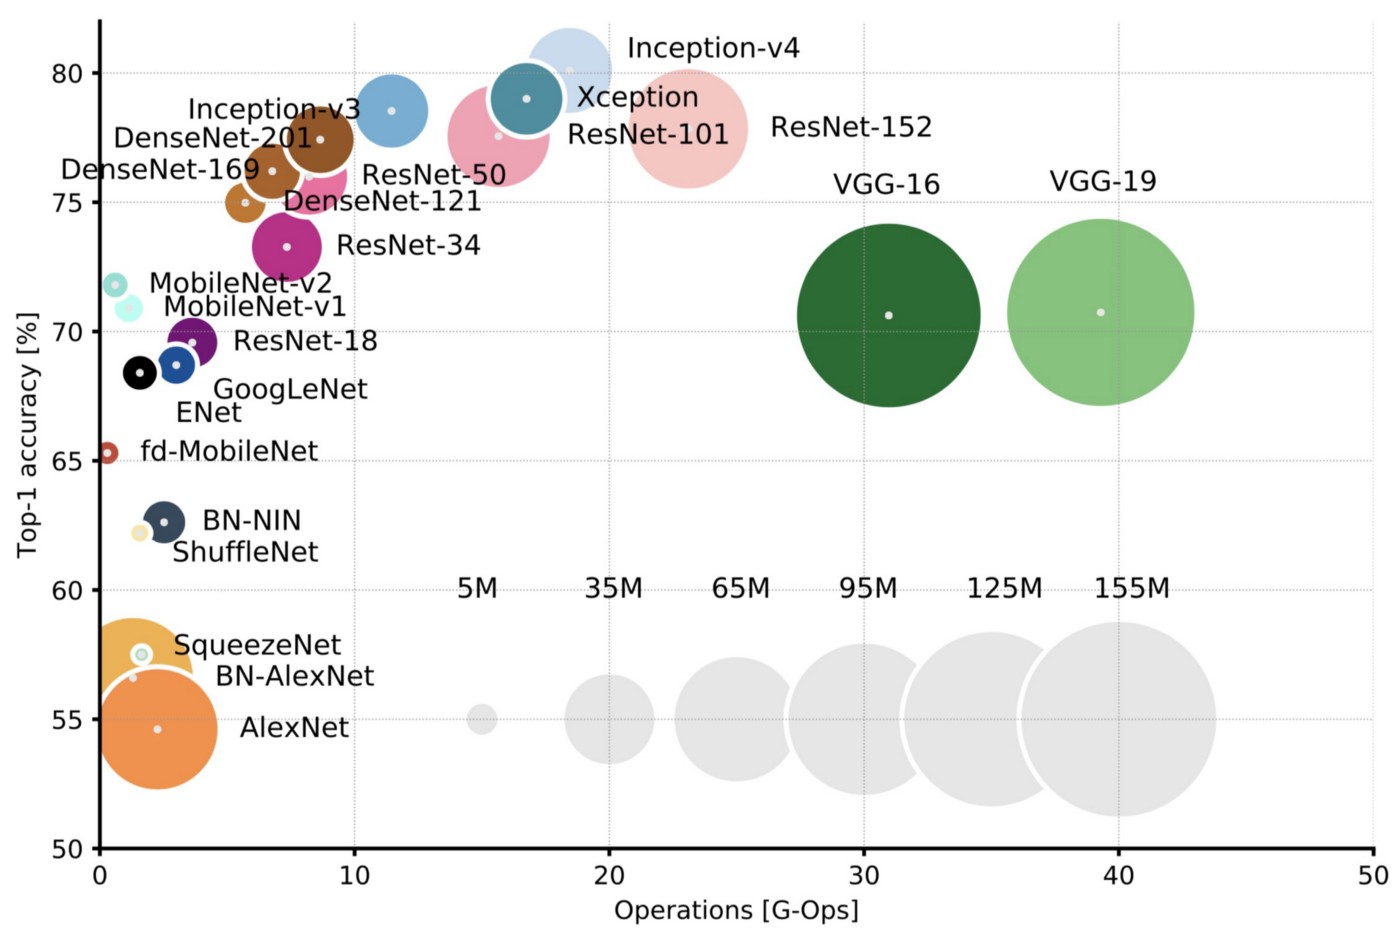
\includegraphics[width=0.8\linewidth]{img/network-comparison.jpeg}
	\caption{Comparison of widely used Image Recognition networks and their performance. Src:TODO: https://arxiv.org/abs/1605.07678}
	\label{fig:camera-setup}
\end{figure}


\section{Distance Measures}

\subsection{Cosine Distance}
\begin{equation}
similarity = \cos ({\bf t},{\bf e})= {{\bf t} {\bf e} \over \|{\bf t}\| \|{\bf e}\|} = \frac{ \sum_{i=1}^{n}{{\bf t}_i{\bf e}_i} }{ \sqrt{\sum_{i=1}^{n}{{\bf t}_i^2}} \sqrt{\sum_{i=1}^{n}{{\bf e}_i^2}} }
\end{equation}
\begin{equation}
    distance = 1 - similarity
\end{equation}

\subsection{Euclidean Distance}
\begin{equation}
d(p, q) = \sqrt{\sum_{i=1}^n (p_i - q_i)^2}    
\end{equation}

\section{Self organizing maps}

\section{?Clustering}

\section{Dataset}

\chapter{Search by Object Location}

First approach we explore is based on knowing the position of the objects in the image. This corresponds to a visual memory. People with a good visual memory are usually able to describe the position of the objects regarding to each other or in absolute way in the whole image. An example to this shows the image \todo[]{}.

We aim to overcome a limitation on vocabulary size for common approach by description of words. We implement search only on visual requests, which, if takes rich enoucgh descriptors has significantly higher capability.

\todo[inline]{Obrazok s hladanou scenou dvoch ludi a k tomu vsetkymi obrazkami kde su dvaja ludia}
\todo[inline]{Obrazok s hladanou scenou dvoch ludi a k tomu kolaz ktora zobrazuje ewquest}

\todo[inline]{Motivation --  spomienka toho, ako vyzerala scena}
\todo[inline]{Now we present following two approaches...}
In the TrackVid competition, many presented solutions are limited and do not scale well. For example is keyword search, which is limited to the size of the vocabulary. In this chapter we overcome this limitation. We develop search based on images instead of words to avoid the vocabulary limit. We use state-of-art knowledge to acquire deep representation of the objects.

The second limitation we tackle is multi-query. It is difficult to find a source video if many scenes with the same type of the objects occur in the dataset (see Image ....). We solve this problem by placing multiple single queries and then using fusion to merge rankings from each query (more in ...).


The research in the recent years showed, that neural networks purposfully trained for a set of objects can gain an ability to create a good representation also for unseen objects \todo[]{source}. In this thesis we work with this presumption and we work with these representations.

\section{Visual Descriptor}
\section{Deep Visual Representations}
--- obfuskavanie sieti

\section{Query}

The query is a collage of one or multiple images. Each image also includes its relative position in the canvas.

The user interacts with the environemnt by adding, scaling and moving images. Interactively, closest representatives found in the dataset are returned. The user can submit if he successfully found the searched scene. The number of hints are taken into account.

The image \todo[]{query image} shows an example of our query. The goal is to be able to use any of currently available image search engines to create a collage. The user places multiple images on the canvas. Their position on the canvas is recorded and later used to target the database in regard to their position. 


\section{Splitting an Image into Regions}



In our first approach we cut the image into fixed regions. We aim to capture the 
representation of each of these regions. This offers us an information specific for each region.

With the query we can compare the features representation of the query and of the particular regions we are interested in.

Image
- Split to nxm regions
- Compute deep representation for each of the regions

Query
compute deep representation for the image in the query
for each image in the database, compare this representation to the representation of the region with highest IoU


In our first approach we split the image to a regions. We compute a deep representation using neural network for each region and the whole image. 
\section{ Using Deep Representation}
   - Using Deep Representation
      = Using antepenultimate layer of classification networks

\section{Multi-query search}
- Multi query search
  - Fusion methods
  - Comparison of both approaches with multimodal performance over different fusion techniques

Our work focuses on difficult to describe scenes with multiple easy to recognize objects. In this questions a natural question of how to rank the results based on multi query.

In this section we go through several approaches we tested. We base our 

\subsection{Fusion Methods}

\section{Evaluation}
In this chapter we evaluate all previously mentioned approached. Firstly, we describe our methodology behind the experiments and then we proceed through all approaches. 

\chapter{Search by Face Similarity}

Research in past several decades proved that human have extreme capability of recognizing the faces. Faces are so special to us as a species, that we are able to ..... We are able to recall that we met specific person dating the meeting years back. Therefore we state a question, if the search based only on faces can be done.

This approach organizes the space of seen faces to help the user to orientate and find the search face. Though, in order to describe the face space we use deep encodings trained by a network used for face recognition.

In the previous chapter we elaborated an approach to search in dataset using objects and their spatial information. In this chapter we investigate a different option -- traversion using faces. The question we ask is if it is possible to find a specific scene by showing user faces. Since there is a limitation of how many faces we can display at once to the user, we will investigate if we can lead user to the specific scene with specific face via traversion through multiple similar faces.

Since the similarity of faces is a strongly abstract perception we rely on feature representation of the faces. This helps us to create an interactive environment to traverse via huge aount of faces and test our hypothesis, if this approach can be used for scene searching. 

This chapter firstly introduces different approaches to obtaining face representations. Then we proceed by presenting different approaches for traversion over dataset of faces. At the end of the chapter we present the results in our specific task -- scene search .

\todo[inline]{ motivation - otestovat hypotezu ci je to mozne a nejaky nahlad ako ot moze vyzerat}
\section{Preliminaries}
\todo[inline]{face features - popisat zdroj siete}
\section{Creating SOM Representation of the face space}
\section{Evaluation}

Appendix
\chapter{User Guide (how to use the app to search)}
\chapter{ Running the app on the new set of images}
\todo[inline]{kde zmenit data a co znova natrenovat}
\chapter{Experiments evaluation (ako ziskat vysledky znova)}
\chapter{Code Structure (programmer's guide)}


% Searching Image Collections Using Deep Representations of Local Regions

% The thesis will investigate two particular approaches for searching large video datasets. The first approach will try to retrieve a searched scene based on a query collage consisting of example images organized on a canvas. The author will investigate various fusion methods, taking into account also the canvas positioning of the query images.  The second approach will be designed to search for a scene based on faces available in the dataset. The method will be based on visual exploration of the faces based on their similarities. In exploration approaches, the user can choose a similar face to the searched one, and continuously browse towards the searched face. The author will provide an interactive search environment for querying as a part of the solution and evaluate the recall on sets of experiments to estimate, how successfully users can retrieve particular scenes.

